%2.3.tex

ベクトル拡張付きRISC-Vは機械語コードが同時演算数に依存しないスケーラブルなベクトル拡張を実現したISAであり,既存のRISC-VをARM SVEを参考にベクトル拡張したものである.
ベクトル拡張付きRISC-Vではスケーラブルなベクトル拡張を行うためにプレディケートによるループ制御がある.プレディケートを用いたループ処理はループカウンタと処理する全データ数を比較してループカウンタが全データ数より小さい間対応するプレディケートレジスタをTrueにする.この命令によってベクトル処理で余りの要素がある場合,余りの要素の部分に対応するプレディケートの要素のみをTrueにする.これによって余りの要素が変化してもすべてのデータ数分ベクトル処理を行うことができ,同時演算数に依存しない機械語コードが実現できる.
プレディケートレジスタの一例を図\ref{fig:predicate}に示す.図\ref{fig:predicate}の(a)ではループカウンタがデータ数より小さい場合であり,プレディケートの要素が全てTrueになっている.図\ref{fig:predicate}の(b)では端数要素の処理を行う場合であり,ループカウンタがデータ数より小さいときのみ要素がTrueとなっている.


\begin{figure}[b]
    \centering
    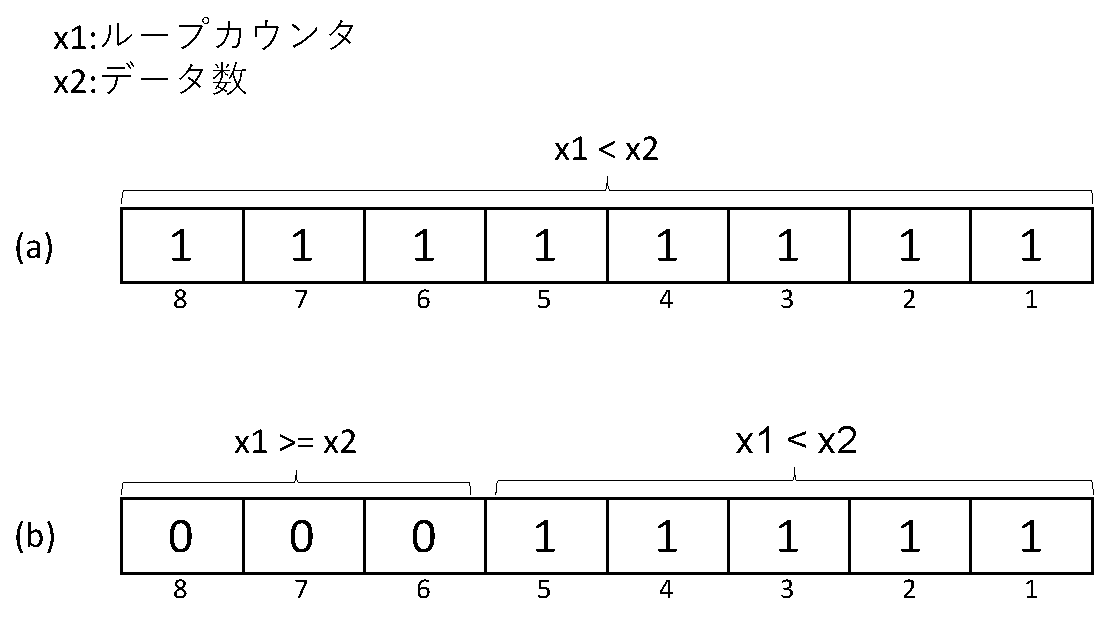
\includegraphics[scale=0.5]{image/predicate.pdf}
    \caption{プレディケートレジスタの一例}
    \label{fig:predicate}
\end{figure}

ベクトル命令はベクトルロード,ストア命令,ベクトル演算命令,ベクトル制御命令の3つに分けられる.RISC-Vにはカスタム命令用にオペコード領域が4つ用意されているがそのうちの2つを利用しており,1つをベクトルロード,ストア命令,もう一方をベクトル演算命令とベクトル制御命令に使用している.ベクトルロード,ストア命令のアドレスはベースとなるスカラレジスタの値にオフセットを加えることで計算する.
ベクトル演算命令は,プレディケートあり演算命令,プレディケートなし演算命令,即値による演算命令に分けられる.
浮動小数点命令は必要なハードウェア資源が多いためサポートしていない.ベクトル拡張付きRISC-Vは基本命令に関してRV32Iのみ組み込んでいる.

レジスタ構成はベクトルレジスタv0-v31,ベクトルマスク制御に用いるためのプレディケートレジスタvp0-vp7,プレディケートレジスタ同士の論理演算に用いるプレディケートレジスタvp8-vp15,RISC-Vの汎用レジスタx0-x31,プログラムカウンタとなっている.ベクトルレジスタの長さは128$\times 2^n(0\leq n\leq 4)$ビットで表され,汎用レジスタの幅は32ビットとなっている.

命令のフォーマットはRISC-Vの命令形式であるR形式に従ったものとなっている.また,デコーダの単純化のために同じフィールドにはできるだけ同じ機能をもたせている.

%図%図入れる
%にベクトル拡張付きRISC-Vのベクトル命令のフォーマットの一例を示す.命令はプレディケートありVADD命令,プレディケートなしVADD命令,即値によるベクトル加算命令であるVADDI,ロード,ストア命令であるVLW,VSW命令である.どの命令もデスティネーションレジスタを指定するためのフィールドは共通となっている.